\documentclass[fleqn]{exam}

\usepackage{fullpage}
\usepackage{enumerate}
\usepackage{unitsdef} 
\usepackage{graphicx}
\usepackage[fleqn]{mathtools}
\usepackage{cancel}
\usepackage{polynom}
\usepackage{float}
\usepackage{mdwlist}
\usepackage{booktabs}
\usepackage{cancel}
\usepackage{polynom}
\usepackage{caption}

\setlength{\mathindent}{.5 cm}

\everymath{\displaystyle}

% \begin{figure}[H]
%   \centering
%   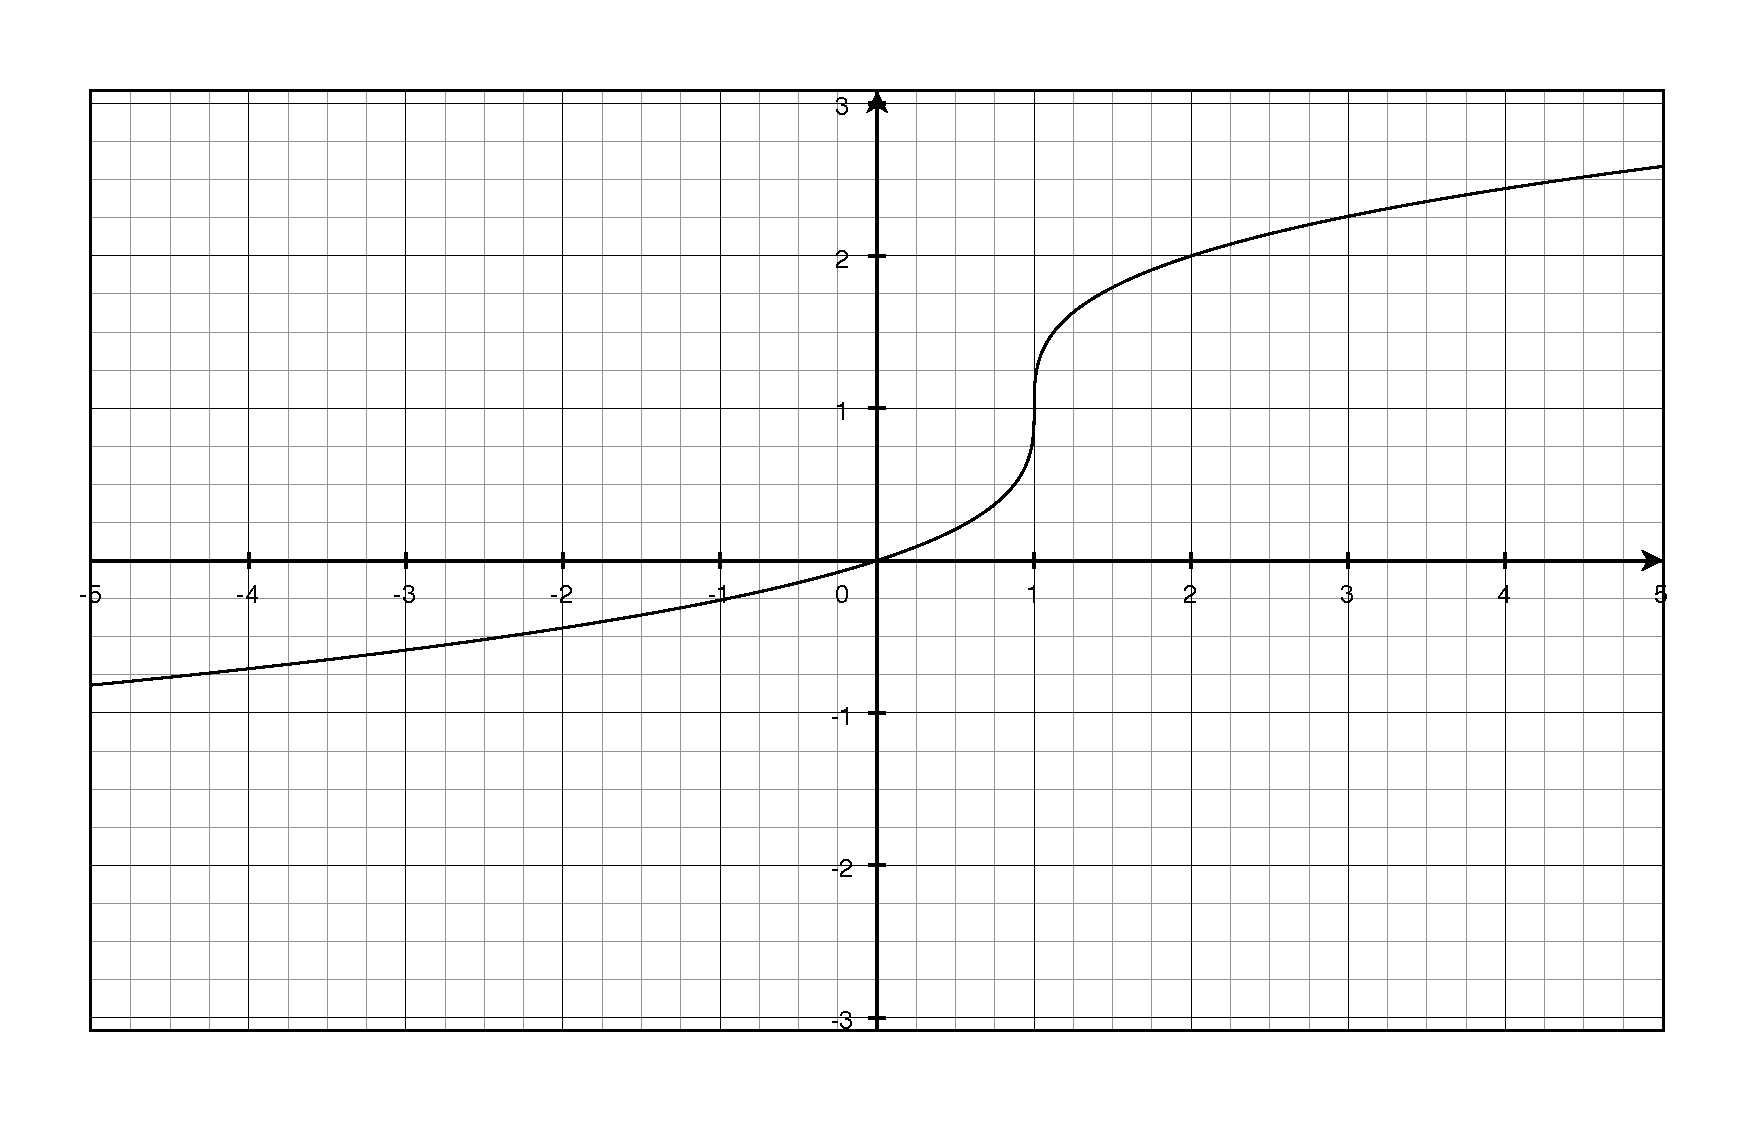
\includegraphics[scale=.3]{question7.eps}
%   \caption*{Question 7}
% \end{figure}

% \begin{tabular}{cc}
% \toprule
% period & amplitude \\
% \midrule
%   $\pi$ & $2$ \\
% \bottomrule
% \end{tabular}

\newunit{\inch}{in}
\newunit{\mile}{mile}
\newunit{\foot}{ft}
\newunit{\knot}{knot}
\newunit{\gallon}{gallon}

\printanswers

\ifprintanswers 
\usepackage{2in1, lscape} 
\fi

\title{Math 263A \\ Homework 15}
\date{May 23, 2012}

\begin{document}

\maketitle

\section{Homework}

\begin{itemize*}
  \item Read Section 4.6
  \item pp. 211-213: 6-15, 17-18, 21-30, 37-38, 41-42
\end{itemize*}

\section{Extra Credit}
\begin{itemize*}
\item page 200, problems 29 and 32
\end{itemize*}

\ifprintanswers
\begin{description}

\item[29]
The distances traveled through each substance are:
\begin{align*}
  d_1 &= \frac{x}{\sin \theta_1} \\
  d_2 &= \frac{d - x}{\sin \theta_2} \\
\end{align*}

The time required to get through both substances is:
\[
  t(x) = \frac{x}{c_1 \sin \theta_1} + \frac{d - x}{c_2 \sin \theta_2} \\ 
\]

To find the minimum, take the derivative and set it to 0:
\begin{align*}
  t'(x) &= \frac{1}{c_1 \sin \theta_1} - \frac{1}{c_2 \sin \theta_2} \\ 
  \frac{1}{c_1 \sin \theta_1} - \frac{1}{c_2 \sin \theta_2} &= 0 \\
  \frac{1}{c_1 \sin \theta_1} &= \frac{1}{c_2 \sin \theta_2} \\ 
  \frac{c_1}{\sin \theta_2} &= \frac{c_2}{\sin \theta_1} \\ 
\end{align*}

We can do a few common-sense checks to see that this relationship makes sense:
\begin{itemize*}
\item if $c_1 = c_2$, then the angles will be equal and the light will travel in a straight line.
\item if one of the two speeds is much larger than the other, its angle is much smaller than the other to compensate.
  This allows the light to minimize the time it spends in the slow substance.
\end{itemize*}

\pagebreak

\item[32]
If we let $x$ be the length of a side of the cube, the paint required is
\begin{itemize}
\item $A_{square} = 6x^2$
\item $A_{sphere} = 1 - 6x^2$
\end{itemize}

We need an expression for the radius of the sphere in terms of the side length of the cube:
\begin{align*}
  4 \pi r^2 &= (1 - 6x^2) \\
  r &= \sqrt{\frac{1 - 6x^2}{4 \pi}} \\
    &= \left(\frac{1 - 6x^2}{4 \pi} \right)^{1/2} \\
\end{align*}

So the volume of the sphere is: 
\begin{align*}
  V_{sphere} &= \frac{4}{3} \pi r^3 \\
  &= \frac{4}{3} \pi \cdot \left(\frac{1 - 6x^2}{4 \pi} \right)^{3/2} \\
\end{align*}

The total volume of the two objects is:
\[
  V = x^3 + \frac{4}{3} \pi \cdot \left(\frac{1 - 6x^2}{4 \pi} \right)^{3/2} \\
\]

Differentiate and set to 0 find the critical points:
\begin{align*}
  V' &= 3x^2 - 6 x \sqrt{\frac{1 - 6x^2}{4 \pi}} \\
\\
  0 &= 3x^2 - 6 x \sqrt{\frac{1 - 6x^2}{4 \pi}} \\
  3x^2 &= 6 x \sqrt{\frac{1 - 6x^2}{4 \pi}} \\
  9x^4 &= 36 x^2 \cdot \left( \frac{1 - 6x^2}{4 \pi} \right) \\
  x &= \sqrt{\frac{1}{\pi + 6}} \\
    &\approx 0.3307 \\
\end{align*}

Check to see if this is a minimum or maximum and what happens if you use all the paint for either the sphere or the square.
\begin{tabular}{rr}
\toprule
x & total volume \\
\midrule
0      & 0.094 \\
0.331  & 0.055 \\
0.408  & 0.068 \\
\bottomrule
\end{tabular}

The minimum volume is with a side length of 0.331 and the maximum volume is achieved by just making a sphere.

\end{description}

\pagebreak

\fi

\section{Review}
\begin{questions}

\question $D_x\left( \frac{3x^2 + 4}{x^3 - 2x} \right)$

\begin{solution}
\begin{align*}
  D_x\left( \frac{3x^2 + 4}{x^3 - 2x} \right) &= \frac{(x^3 - 2x)(6x) - (3x^2 + 4)(3x^2 - 2)}{(x^3 - 2x)^2} \\
  &= \frac{6x^4 - 12x^2 - (9x^4 + 6x^2 - 8)}{(x^3 - 2x)^2} \\
  &= \frac{-3x^4 - 18x^2 + 8}{(x^3 - 2x)^2} \\
\end{align*}

\end{solution}

\question $D_{\theta} \cos \theta^2$

\begin{solution}
\[
  D_{\theta} \cos \theta^2 = D_{\theta} \cos \left( \theta^2 \right) 
    = -\sin \theta^2 \cdot 2 \theta = -2 \theta \sin \theta^2
\]
\end{solution}

\question $D_{\theta} \cos^2 \theta$
\begin{solution}
\[
  D_{\theta} \cos^2 \theta = D_{\theta} \left(\cos \theta \right)^2
    = 2 \cos \theta \cdot (- \sin \theta) = -2 \sin \theta \cos \theta
\]
\end{solution}

\ifprintanswers
\pagebreak
\fi

\question $D_{\theta} \cos^2 \theta^2$

\begin{solution}
\begin{align*}
  D_{\theta} \cos^2 \theta^2 &= D_{\theta} \left(\cos (\theta^2) \right)^2 \\
  &= 2 \cos \theta^2 \cdot D_x \cos \theta^2 \\
  &= 2 \cos \theta^2 \cdot (-2 \theta \sin \theta^2) \\
  &= -4 \theta \sin \theta^2 \cos \theta^2 \\  
\end{align*}

\end{solution}

% \question $D_x \left( \frac{3x \sin x}{\cos x + \sin x} \right)$

% \begin{solution}

% \begin{align*}
%   D_x & \left( \frac{3x \sin x}{\cos x + \sin x} \right) \\
%     &= 3 \cdot \frac{(\cos x + \sin x)(x \cos x + \sin x) - x \sin x (- \sin x + \cos x)}{(\sin x + \cos x)^2} \\  
%     &= 3 \cdot \frac{x \cos^2 x + x \sin x \cos x + \sin x \cos x + \sin^2 x + x \sin^2 x - x \sin x \cos x}{(\sin x + \cos x)^2} \\  
%     &= 3 \cdot \frac{x(\sin^2 x + \cos^2 x) + \sin x \cos x + \sin^2 x}{(\sin x + \cos x)^2} \\  
%     &= 3 \cdot \frac{x + \sin x \cos x + \sin^2 x}{(\sin x + \cos x)^2} \\  
% \end{align*}

% \end{solution}

\question $D_x \left( \frac{\cot x}{\sec x^2} \right)$

\begin{solution}
\begin{align*}
  D_x \left( \frac{\cot x}{\sec x^2} \right) &= D_x \left( \cot x \cos x^2 \right) \\
  &= \cot x \left(- \sin x^2 \right)(2x) + \cos x^2 (- \csc x) \\
  &= -2x \cot x \sin x^2 - \csc^2 x \cos x^2 \\
\end{align*}

\end{solution}
\end{questions}

\ifprintanswers
\pagebreak

\section{Section 4.6}

\begin{description}

\item[6]
\[
  \lim_{x \to \infty} \frac{x^2}{x^2 - 8x + 15} = \lim_{x \to \infty} \frac{1}{1 - \frac{8}{x} + \frac{15}{x^2}} = 1
\]

\item[7]
\[
  \lim_{x \to \infty} \frac{x^3}{2x^3 - 100x^2} = \lim_{x \to \infty} \frac{1}{2 - \frac{100}{x}} = \frac{1}{2} 
\]

\item[8]
\[
  \lim_{\theta \to \infty} \frac{\pi \theta^5}{\theta^5 - 5 \theta^4} =   \lim_{\theta \to \infty} \frac{\pi}{1 - \frac{5}{\theta}} = \pi
\]

\item[9]
\[
  \lim_{x \to \infty} \frac{3x^3 - x^2}{\pi x^3 - 5x^2} = \lim_{x \to \infty} \frac{3 - \frac{1}{x}}{\pi - \frac{5}{x}} = \frac{3}{\pi}
\]

\item[10]
\[
  \lim_{\theta \to \infty} \frac{\sin^2 \theta}{\theta^2 - 5} = 0
\]
The denominator gets larger and larger while the numerator stays between 0 and 1.

\item[11]
\[
  \lim_{x \to \infty} \frac{3 x^{3/2} + 3x}{\sqrt{2} x^{3/2}} = \lim_{x \to \infty} \frac{3 + 3 x^{-1/2}}{\sqrt{2}} = \frac{3}{\sqrt{2}}
\]

\item[12]
\[
  \lim_{x \to \infty} \sqrt[3]{ \frac{\pi x^3 + 3x}{\sqrt{2} x^3 + 7x} } 
  = \lim_{x \to \infty} \sqrt[3]{ \frac{\pi + \frac{3}{x^2}}{\sqrt{2} + \frac{7}{x^2}}} 
  = \sqrt[3]{ \frac{\pi}{\sqrt{2}} } 
  = \frac{\sqrt[3]{\pi}}{\sqrt[6]{2}}
\]

\item[13]
\[
  \lim_{x \to \infty} \sqrt[3]{ \frac{1 + 8x^2}{x^2 + 4} }
  = \lim_{x \to \infty} \sqrt[3]{ \frac{ \frac{1}{x^2} + 8}{1 + \frac{4}{x^2}} }
  = \sqrt[3]{8}
  = 2
\]

\item[14]
\begin{align*}
  \lim_{x \to \infty} \sqrt[3]{ \frac{x^2 + x + 3}{(x - 1)(x + 1)} } &= \lim_{x \to \infty} \sqrt[3]{ \frac{x^2 + x + 3}{x^2 - 1} } \\
  &= \lim_{x \to \infty} \sqrt[3]{ \frac{1 + \frac{1}{x} + \frac{3}{x^2}}{1 - \frac{1}{x^2}} } \\
  &= 1 \\
\end{align*}

\item[15]
\[
  \lim_{x \to \infty} \frac{2x + 1}{\sqrt{x^2 + 3}} = \lim_{x \to \infty} \frac{2 + \frac{1}{x}}{\sqrt{1 + \frac{3}{x^2}}} = 2
\]

\item[17]
\begin{align*}
  \lim_{x \to \infty} &\left( \sqrt{2x^2 + 3} - \sqrt{2x^2 - 5} \right) \\
  &= \lim_{x \to \infty} \left[ \left(\sqrt{2x^2 + 3} - \sqrt{2x^2 - 5} \right) \cdot \frac{\sqrt{2x^2 + 3} + \sqrt{2x^2 - 5}}{\sqrt{2x^2 + 3} + \sqrt{2x^2 - 5}} \right] \\
  &= \lim_{x \to \infty} \frac{2x^2 + 3 - (2x^2 - 5)}{\sqrt{2x^2 + 3} + \sqrt{2x^2 - 5}}) \\
  &= \lim_{x \to \infty} \frac{8}{\sqrt{2x^2 + 3} + \sqrt{2x^2 - 5}}) \\
  &= 0 \\
\end{align*}

\item[18]
\begin{align*}
  \lim_{x \to \infty} \left( \sqrt{x^2 + 2x} - x \right)
  &= \lim_{x \to \infty} \left[ \left(\sqrt{x^2 + 2x} - x \right) \cdot \frac{\sqrt{x^2 + 2x} + x}{\sqrt{x^2 + 2x} + x} \right] \\
  &= \lim_{x \to \infty} \frac{x^2 + 2x - x^2}{\sqrt{x^2 + 2x} + x} \\
  &= \lim_{x \to \infty} \frac{2x}{\sqrt{x^2 + 2x} + x} \\
  &= \lim_{x \to \infty} \frac{2}{\sqrt{1 + \frac{2}{x}} + 1} \\
  &= 1 \\
\end{align*}

\item[21]
\[
  \lim_{x \to 4^+} \frac{x}{x - 4} = \infty
\]

\item[22]
\[
  \lim_{t \to -3^+} \frac{t^2 - 9}{t + 3} = \lim_{t \to -3^+} \frac{(t + 3)(t - 3)}{t + 3} = \lim_{t \to -3^+} (t - 3) = -6
\]

\item[23]
\[
  \lim_{t \to 3^-} \frac{t^2}{9 - t^2} = \infty
\]

\item[24]
\[
  \lim_{x \to \sqrt[3]{5}^+} \frac{x^2}{5 - x^3} = -\infty
\]

\item[25]
\[
  \lim_{x \to 5^-} \frac{x^2}{(x - 5)(3 - x)} = \infty
\]

\item[26]
\[
  \lim_{\theta \to \pi^+} \frac{\theta^2}{\sin \theta} = - \infty
\]

\item[27]
\[
  \lim_{x \to 3^-} \frac{x^3}{x - 3} = - \infty
\]

\item[28]
\[
  \lim_{x \to (\pi/2)^+} \frac{\pi \theta}{\cos \theta} = -\infty
\]

\item[29]
\[
  \lim_{x \to 3^-} \frac{x^2 - x - 6}{x - 3} = \lim_{x \to 3^-} \frac{(x + 2)(x - 3)}{x - 3} = \lim_{x \to 3^-} (x + 2) = 5
\]

\item[30]
\[
  \lim_{x \to 2^+} \frac{x^2 + 2x - 8}{x^2 - 4} = \lim_{x \to 2^+} \frac{(x - 2)(x + 4)}{(x + 2)(x - 2)} = \lim_{x \to 2^+} \frac{x + 4}{x + 2} = \frac{3}{2}
\]

\pagebreak

\item[37]
horizontal asymptote:
\[
  \lim_{x \to \infty} \frac{3}{x + 1} = \lim_{x \to -\infty} \frac{3}{x + 1} = 0
\]

vertical asymptote
\begin{align*}
  \lim_{x \to -1^+} \frac{3}{x + 1} &= \infty \\
  \lim_{x \to -1^-} \frac{3}{x + 1} &= -\infty \\
\end{align*}

\begin{figure}[H]
  \centering
  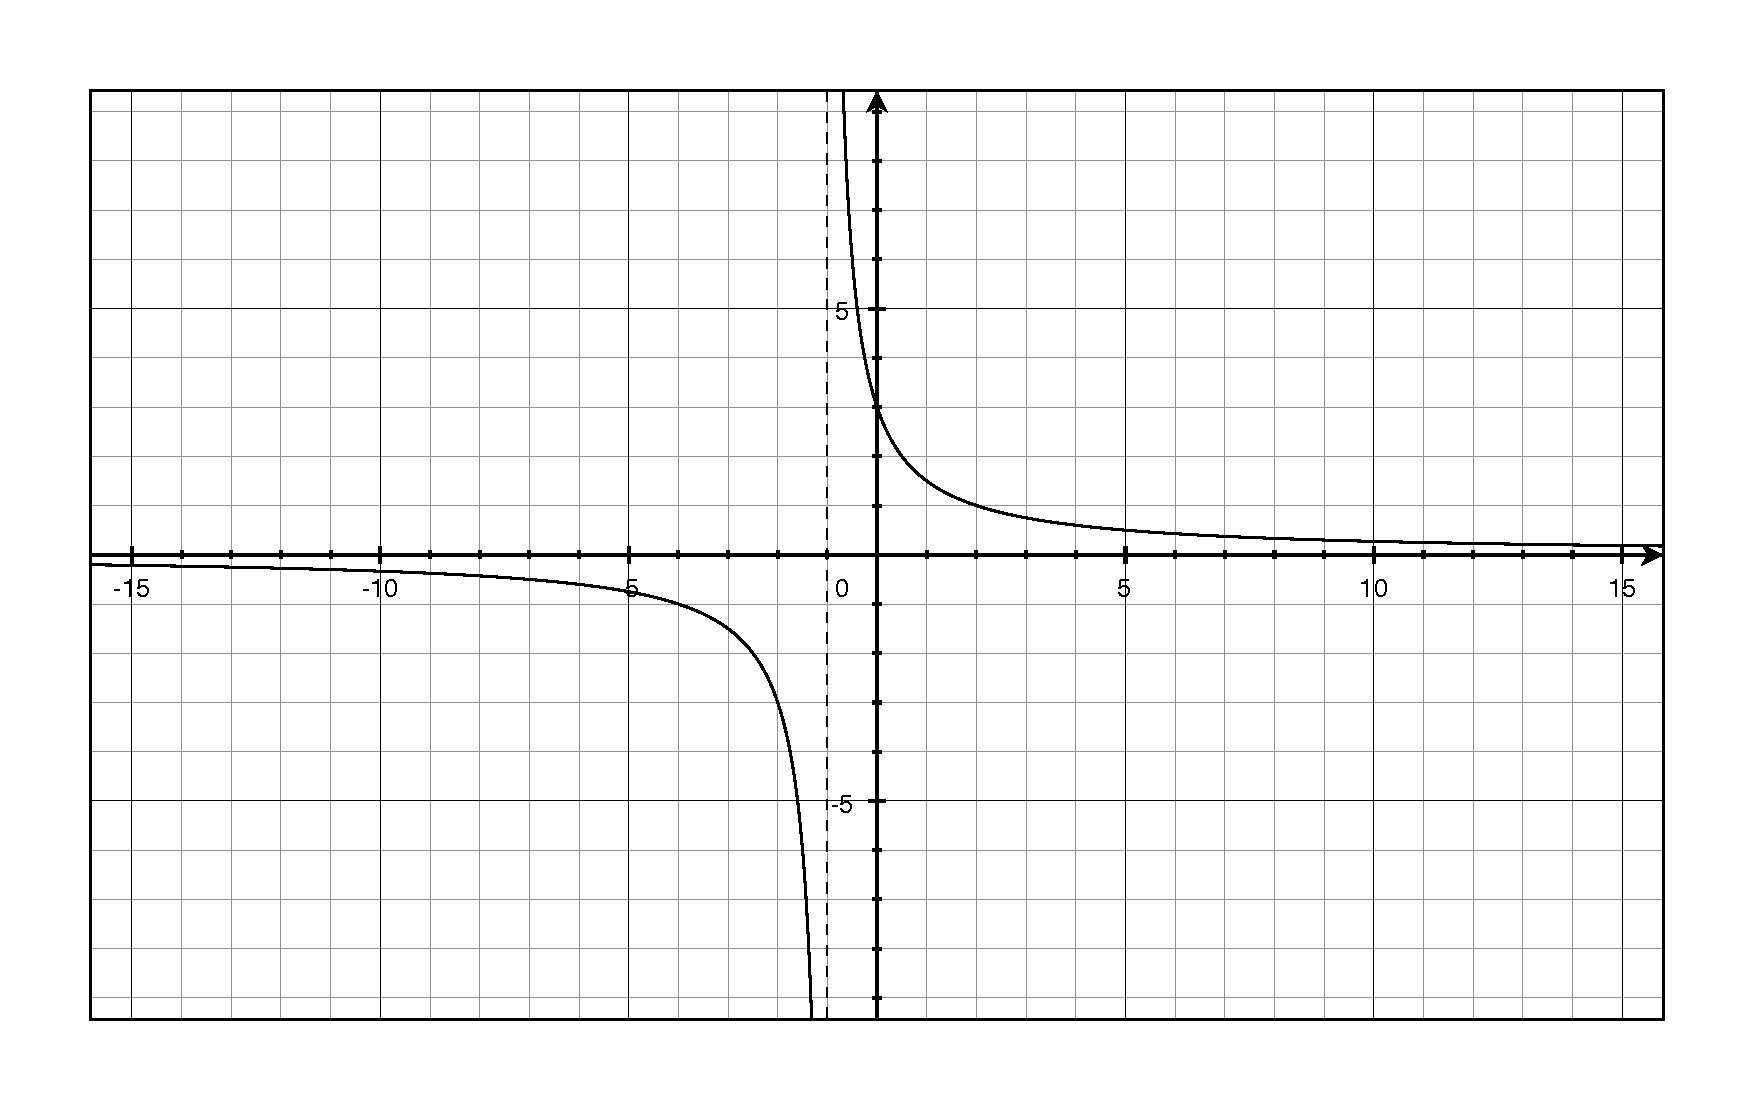
\includegraphics[scale=.3]{problem_37.eps}
  \caption*{Problem 37}
\end{figure}

\pagebreak

\item[38]

horizontal asymptote:
\[
  \lim_{x \to \infty} \frac{3}{(x + 1)^2} = \lim_{x \to -\infty} \frac{3}{(x + 1)^2} = 0
\]

vertical asymptote
\[
  \lim_{x \to -1} \frac{3}{(x + 1)^2} = \infty
\]

\begin{figure}[H]
  \centering
  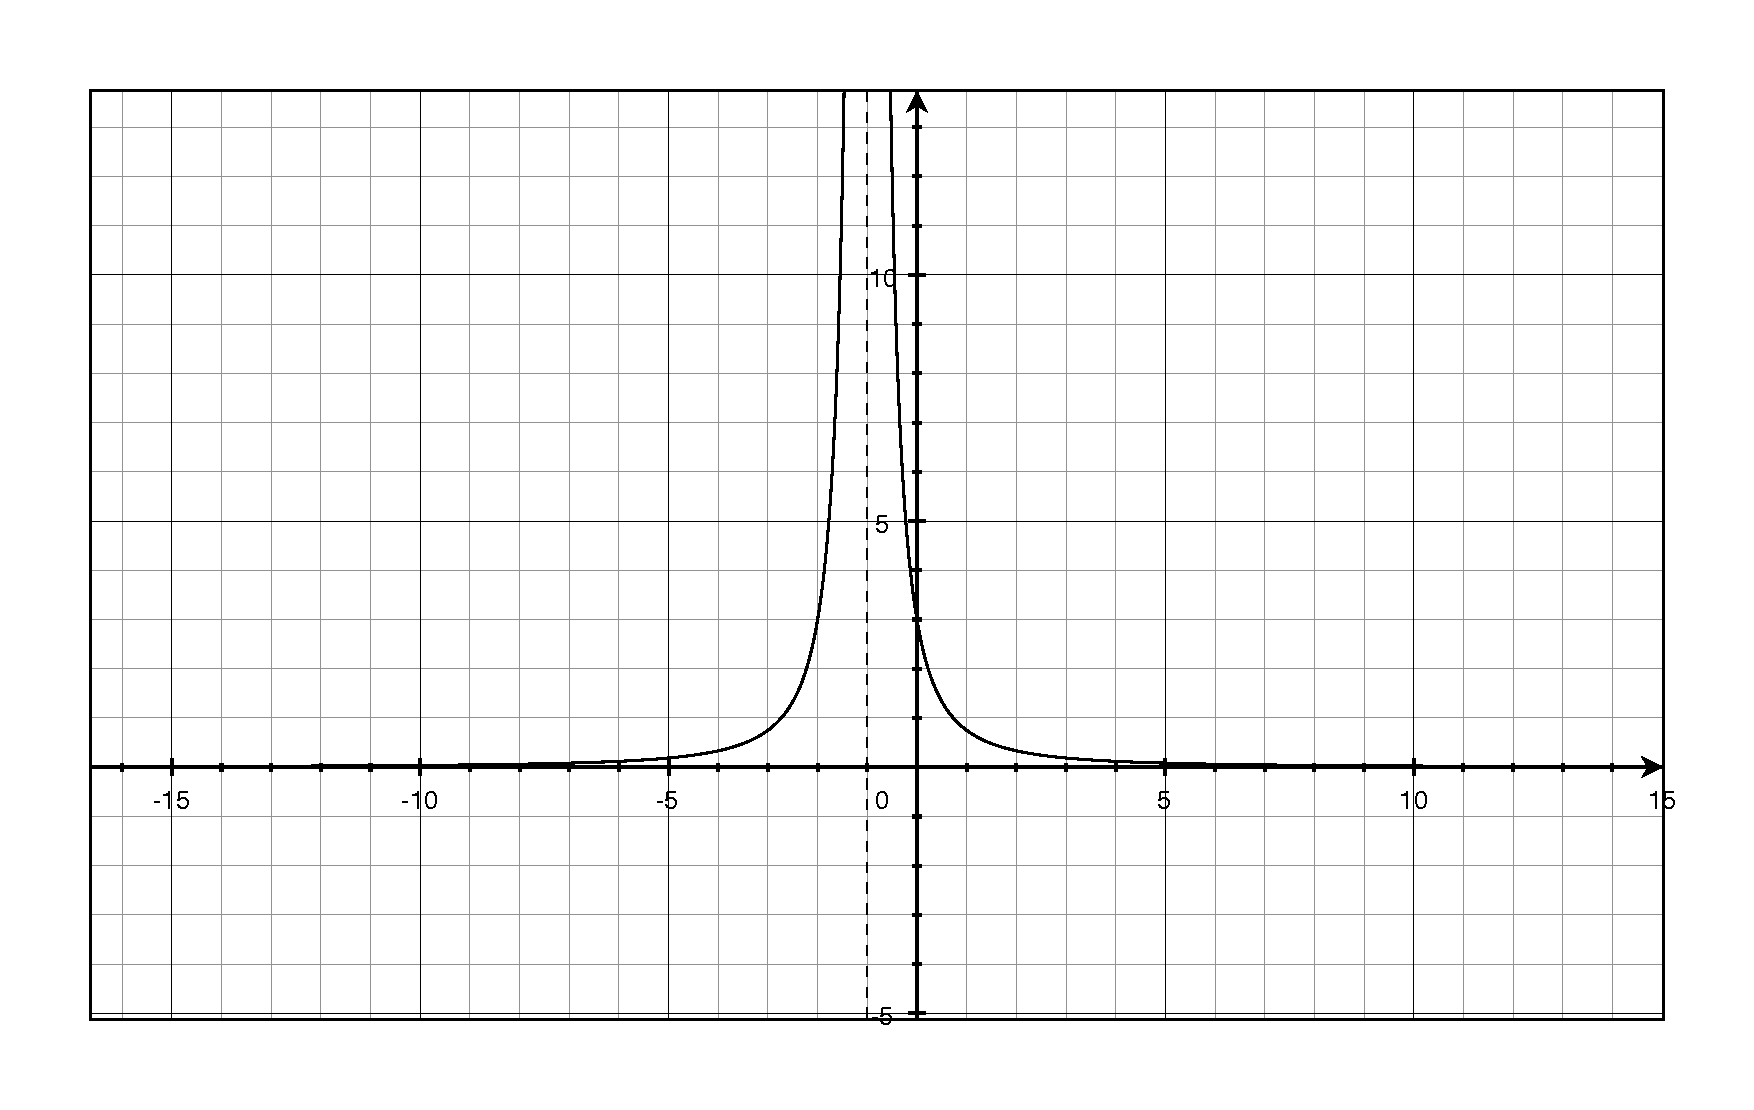
\includegraphics[scale=.3]{problem_38.eps}
  \caption*{Problem 38}
\end{figure}

\pagebreak

\item[41]

horizontal asymptote:
\[
  \lim_{x \to \infty} \frac{14}{2x^2 + 7} = \lim_{x \to -\infty} \frac{14}{2x^2 + 7} = 0
\]

no vertical asymptote since the denominator can never be zero.

%% We can use the first derivative test to find out where the function is increasing:
%% \[
%%   f'(x) = \frac{-14(4x)}{(2x^2 + 7)^2} = \frac{-56x}{(2x^2 + 7)^2}
%% \]

%% $f$ increases in$(-\infty, 0)$ and decreases in $(0, \infty)$.

\begin{figure}[H]
  \centering
  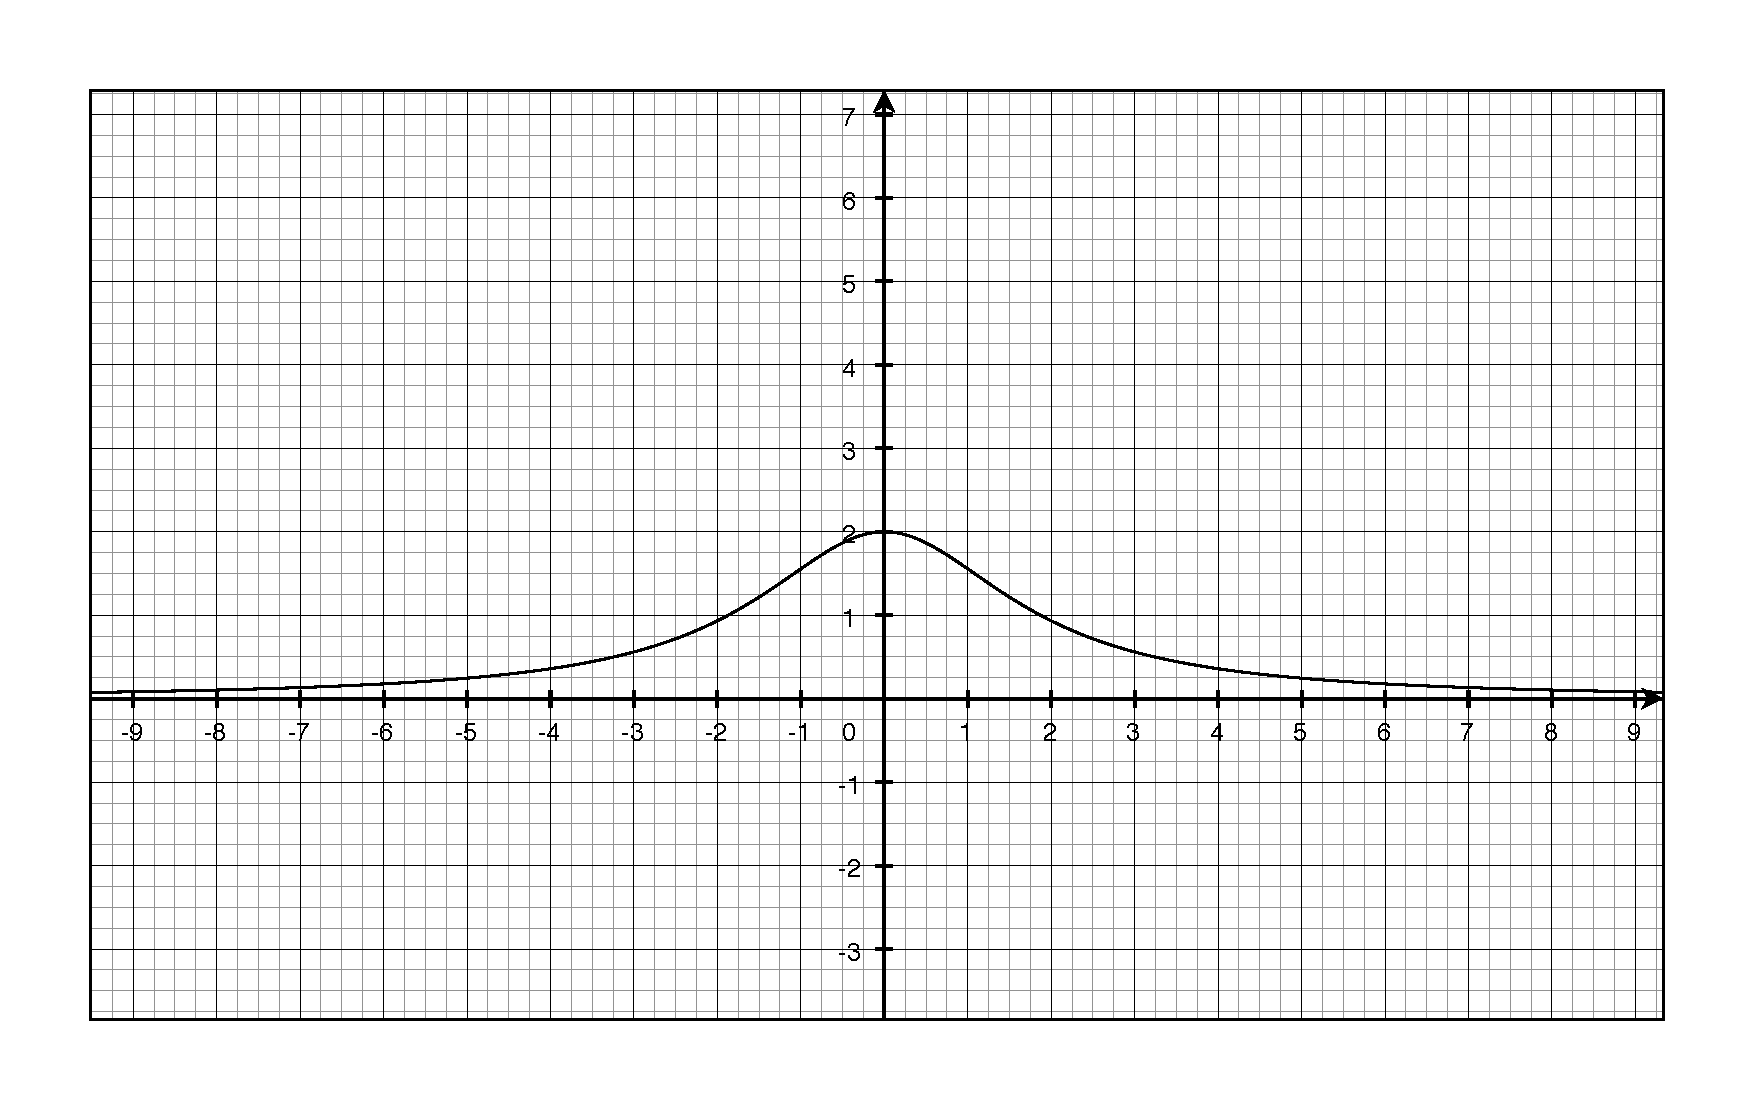
\includegraphics[scale=.3]{problem_41.eps}
  \caption*{Problem 41}
\end{figure}

\pagebreak

\item[42]

horizontal asymptotes:
\begin{align*}
  \lim_{x \to \infty} \frac{2x}{\sqrt{x^2 + 5}} &= \lim_{x \to \infty} \frac{2}{\sqrt{1 + \frac{5}{x^2}}} = 2 \\
  \lim_{x \to -\infty} \frac{2x}{\sqrt{x^2 + 5}} &= \lim_{x \to \infty} \frac{-2}{\sqrt{1 + \frac{5}{x^2}}} = -2 \\
\end{align*}

no vertical asymptote since the denominator can never be zero.

$f$ increases in$(-\infty, 0)$ and decreases in $(0, \infty)$.

\begin{figure}[H]
  \centering
  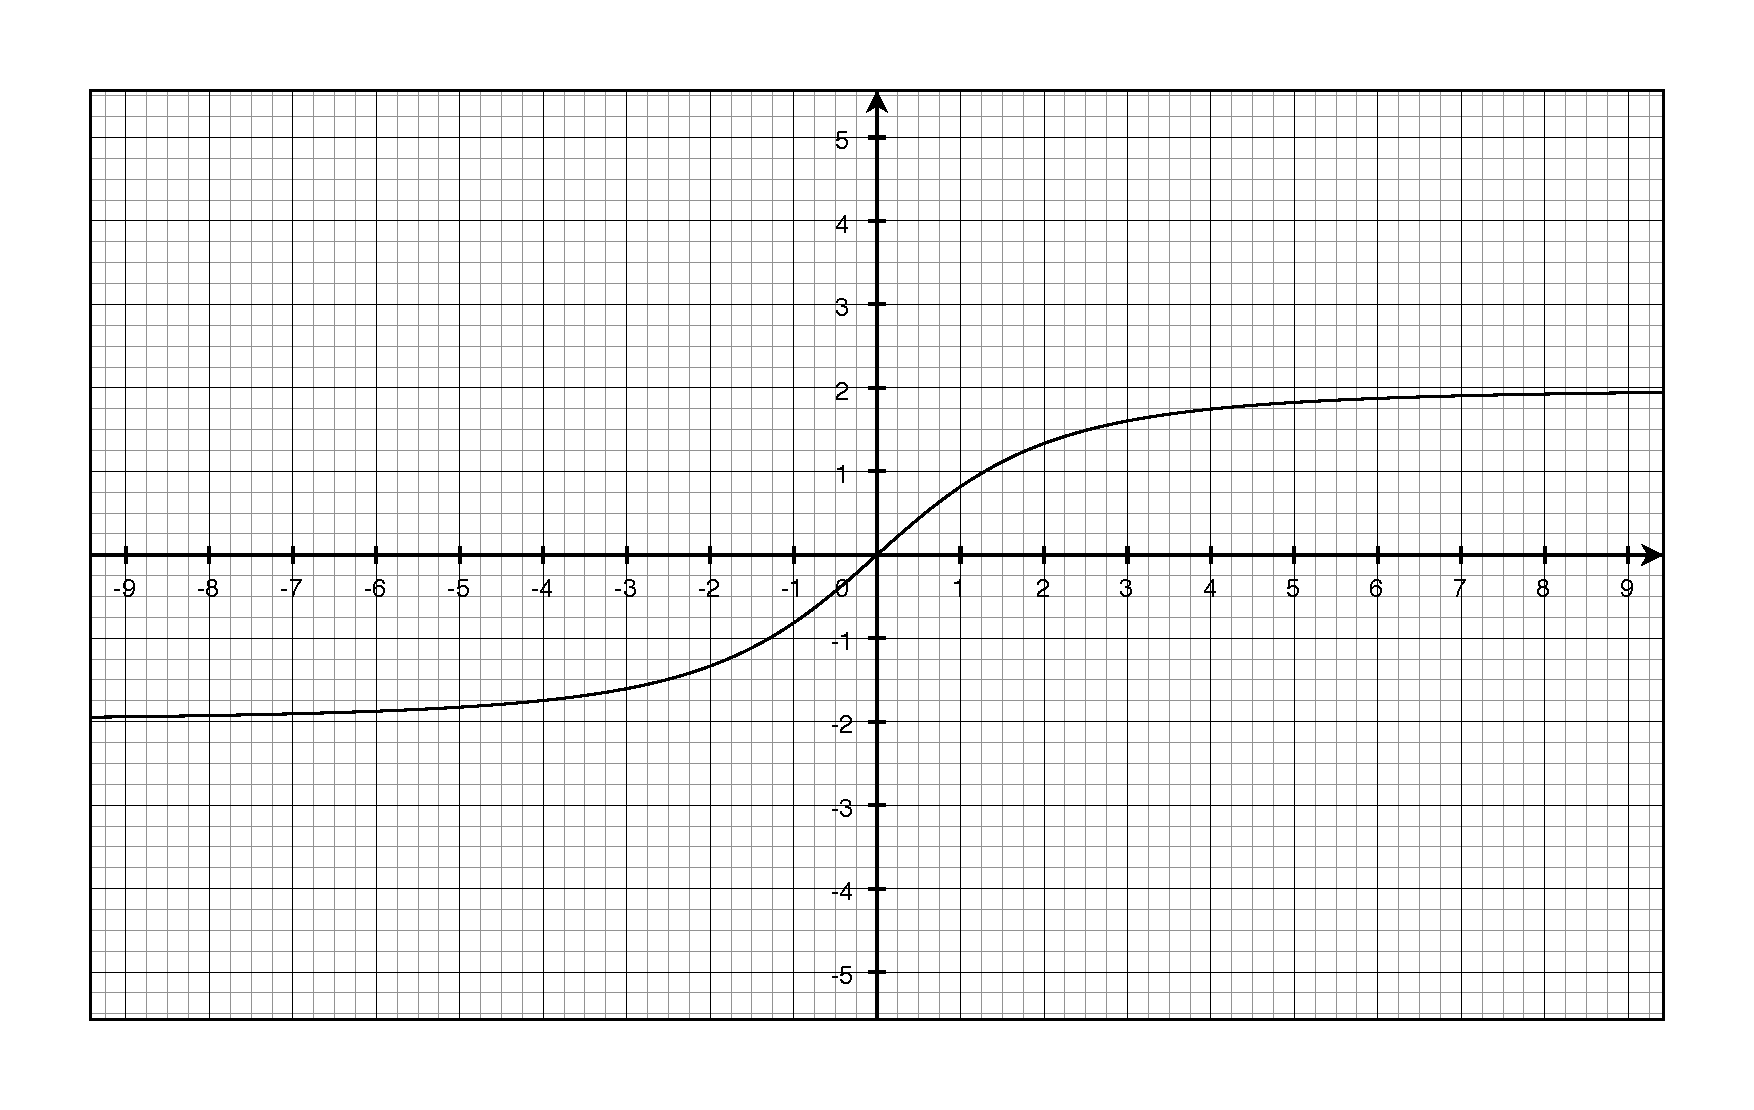
\includegraphics[scale=.3]{problem_42.eps}
  \caption*{Problem 42}
\end{figure}

%% \item[49]
%% \begin{enumerate}[a]

%% \item $\lim_{x \to \infty} \sin x$ is not defined since $f$ doesn't approach any particular number as $x$ gets larger and larger.

%% \item $\lim_{x \to \infty} \sin \frac{1}{x} = 0$

%% \item 
%% \[
%%   \lim_{x \to \infty} x \sin \frac{1}{x} = \lim_{x \to 0} \frac{\sin x}{x} = 1
%% \]

%% \item 
%% \[
%%   \lim_{x \to \infty} x^{3/2} \sin \frac{1}{x} = \lim_{x \to 0} \frac{\sin x}{x} \cdot \lim_{x \to 0} x^{-1/2}
%% \]

%% \end{enumerate}

\end{description}

\else

\vspace{4 cm}

{\em Must the citizen ever for a moment, or in the least degree, resign his conscience to the legislator? Why has every
  man a conscience, then? I think that we should be men first, and subjects afterward. It is not desirable to cultivate
  a respect for the law, so much as for the right.}

\vspace{.2 cm}

\hspace{1 cm} --Henry David Thoreau

\fi

\end{document}

